\documentclass{beamer}

\usepackage[utf8x]{inputenc}
\usepackage[OT4]{fontenc}

\usetheme[bullet=circle,
          titleline=true,
          pageofpages=of,
          alternativetitlepage=true]{Torino}

\usepackage{color}

\usepackage{ragged2e}
\usepackage{hyphenat}
\usepackage{booktabs}

\usepackage{tikz}

\usetikzlibrary{arrows}
\usetikzlibrary{automata}
\usetikzlibrary{backgrounds}
\usetikzlibrary{decorations}

\usepackage{amsmath}
\usepackage{amsfonts}
\usepackage{amsthm}

\usepackage{../../slides/highlight/axiomhighlight}
\usepackage{../../slides/highlight/maximahighlight}
\usepackage{../../slides/highlight/pythonhighlight}
\usepackage{../../slides/highlight/mathematicahighlight}

\definecolor{MyGreen}{rgb}{0.40,0.80,0.20}

\title{Symbolic manipulation in pure Python. Is it feasible?}
\author{Mateusz Paprocki \texttt{<mattpap@gmail.com>}}
\institute[PWR]{Wrocław University of Technology \linebreak SymPy Development Team}
\date{\today}

\newenvironment{jblock}[1]{
    \begin{block}{#1}\justifying\nohyphens
}{
    \end{block}
}

\begin{document}

\setbeamercovered{transparent}

\frame{\titlepage}

\begin{frame}[fragile]
    \frametitle{Presentation plan}

    \begin{itemize}
        \item A few words about the author
        \pause
        \item Short introduction to SymPy
            \begin{itemize}
                \item the main goals of the project
                \item listing of SymPy's capabilities
            \end{itemize}
        \pause
        \item The main topic
            \begin{itemize}
                \item polynomials in SymPy
                \item compare with other systems
                \item examples, more examples \ldots
            \end{itemize}
    \end{itemize}
\end{frame}

\begin{frame}[fragile]
    \frametitle{A few words about the author}

    \begin{center}
        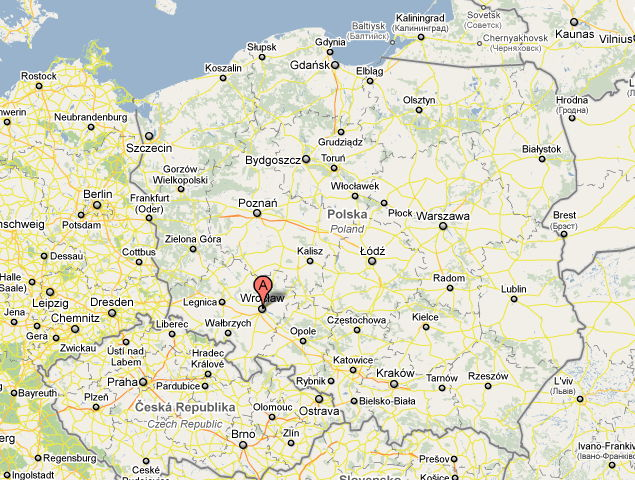
\includegraphics[scale=0.6]{images/wr1.jpg}
    \end{center}
\end{frame}

\begin{frame}[fragile]
    \frametitle{Wrocław University of Technology (1)}

    \begin{center}
        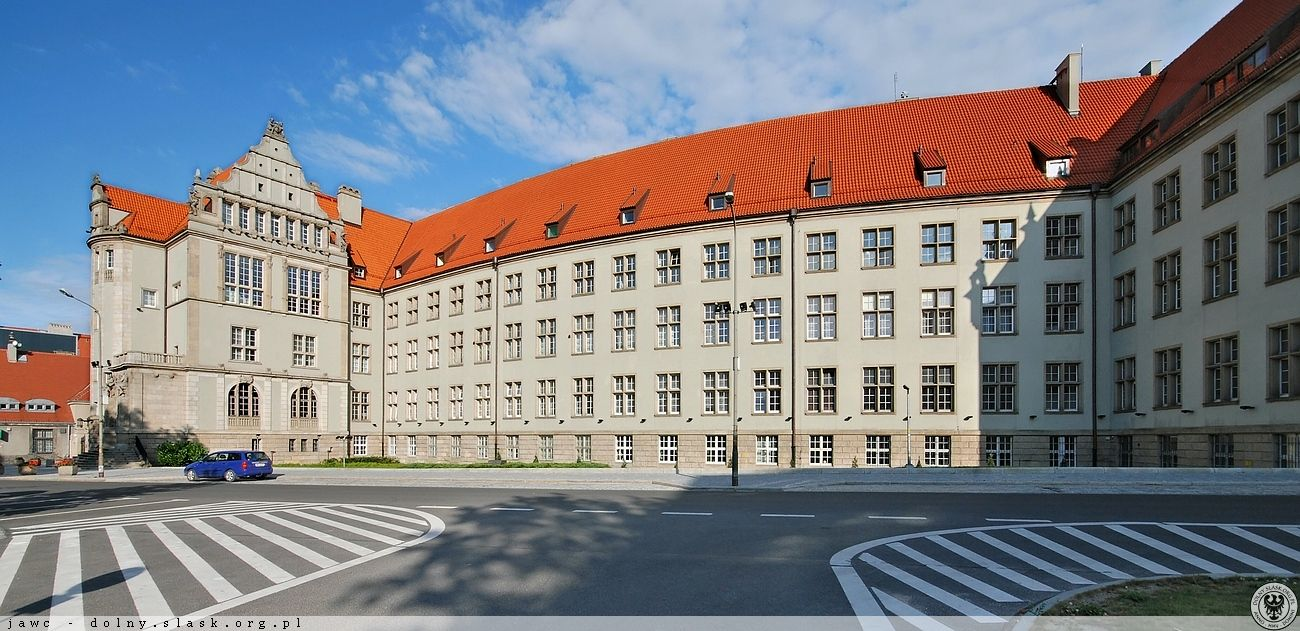
\includegraphics[scale=0.25]{images/pwr1.jpg}
    \end{center}
\end{frame}

\begin{frame}[fragile]
    \frametitle{Wrocław University of Technology (2)}

    \begin{center}
        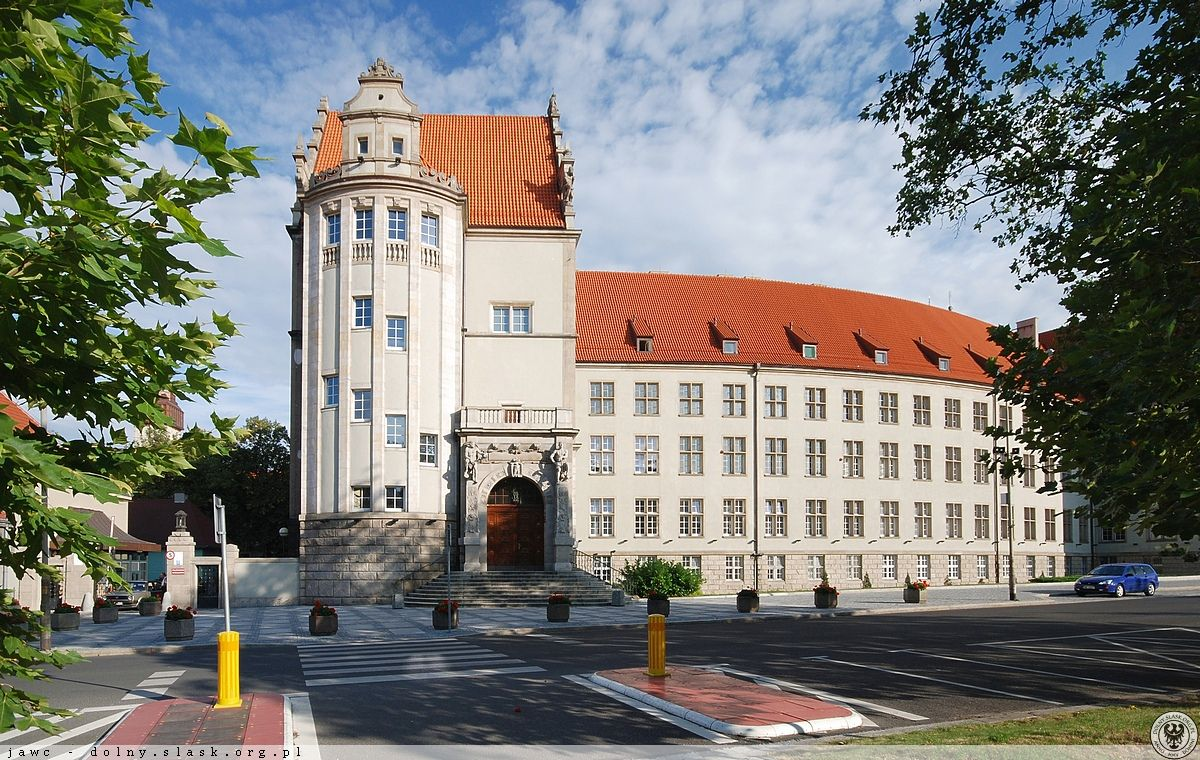
\includegraphics[scale=0.25]{images/pwr2.jpg}
    \end{center}
\end{frame}

\begin{frame}[fragile]
    \frametitle{What is SymPy?}

    \begin{itemize}
        \item A pure Python library for symbolic mathematics
    \end{itemize}

    \pause
    \begin{python}
  >>> from sympy import *
  >>> x = Symbol('x')

  >>> limit(sin(pi*x)/x, x, 0)
  pi

  >>> integrate(x + sinh(x), x)
  (1/2)*x**2 + cosh(x)

  >>> diff(_, x)
  x + sinh(x)
    \end{python}
\end{frame}

\begin{frame}
    \frametitle{My role in the project}
    \framesubtitle{A short historical background}

    \begin{itemize}
        \item cooperation started in March 2007
            \begin{itemize}
                \item a few simple bugfixes and improvements
            \end{itemize}
            \pause
        \item next came Google Summer of Code 2007
            \begin{itemize}
                \item algorithms for solving recurrence relations
                \item algorithms for definite and indefinite summations
            \end{itemize}
            \pause
        \item and this is how it works:
            \begin{itemize}
                \item algorithms for symbolic integration
                \item algebraic structures, polynomials
                \item expression simplification, \ldots
            \end{itemize}
            \pause
        \item else:
            \begin{itemize}
                \item GSoC 2009, 2010 mentor (PSU, PSF)
                \item tutorial at EuroSciPy '09
                \item master's thesis
            \end{itemize}
    \end{itemize}
\end{frame}

\begin{frame}[fragile]
    \frametitle{Why reinvent the wheel for the 37th time?}

    There are numerous symbolic manipulation systems:
    \begin{itemize}
        \item \structure{Proprietary} software:
            \begin{itemize}
                \item Mathematica, Maple, Magma, \ldots
            \end{itemize}
        \item \structure{Open Source} software:
            \begin{itemize}
                \item AXIOM, GiNaC, Maxima, PARI, Sage, Singular, Yacas, \ldots
            \end{itemize}
    \end{itemize}
    \pause
    {\color{red} Problems:}
    \begin{itemize}
        \item all \structure{invent} their own \structure{language}
            \begin{itemize}
                \item need to learn yet another language
                \item separation into core and library
                \item hard to extend core functionality
                \item \structure{except}: GiNaC and Sage
            \end{itemize}
        \item all need quite some time to compile
            \begin{itemize}
                \item slow development cycle
            \end{itemize}
    \end{itemize}
\end{frame}

\begin{frame}[fragile]
    \frametitle{List of SymPy's modules (1)}

    \begin{description}
        \item[concrete] symbolic products and summations
        \item[core] Basic, Add, Mul, Pow, Function, \structure{\ldots}
        \item[functions] elementary and special functions
        \item[galgebra] geometric algebra
        \item[geometry] geometric entities
        \item[integrals] symbolic integrator
        \item[interactive] for setting up pretty--printing
        \item[logic] new assumptions engine, boolean functions
        \item[matrices] Matrix class, orthogonalization etc.
        \item[mpmath] fast arbitrary precision numerical math
    \end{description}
\end{frame}

\begin{frame}[fragile]
    \frametitle{List of SymPy's modules (2)}

    \begin{description}
        \item[ntheory] number theoretical functions
        \item[parsing] Mathematica and Maxima parsers
        \item[physics] physical units, Pauli matrices
        \item[plotting] 2D and 3D plots using pyglet
        \item[polys] polynomial algebra, factorization
        \item[printing] pretty-printing, code generation
        \item[series] compute limits and tructated series
        \item[simplify] rewrite expresions in other forms
        \item[solvers] algebraic, recurrence, differential
        \item[statistics] standard probability distributions
        \item[utilities] test framework, compatibility stuff
    \end{description}
\end{frame}

\begin{frame}[fragile]
    \frametitle{How to get involved?}

    \begin{itemize}
        \item Visit our main web site:
            \begin{itemize}
                \item \texttt{www.sympy.org}
            \end{itemize}
        \item and additional web sites:
            \begin{itemize}
                \item \texttt{docs.sympy.org}
                \item \texttt{wiki.sympy.org}
                \item \texttt{live.sympy.org}
            \end{itemize}
        \item Contact us on our mailing list:
            \begin{itemize}
                \item \texttt{sympy@googlegroups.com}
            \end{itemize}
        \item or/and IRC channel:
            \begin{itemize}
                \item \texttt{\#sympy} on FreeNode
            \end{itemize}
        \item Clone source repository:
        \begin{verbatim}
        git clone git://git.sympy.org/sympy.git
        \end{verbatim}
    \end{itemize}
\end{frame}

\begin{frame}
    \frametitle{The first example}
    \framesubtitle{Vertex $k$--coloring of graphs}

    \begin{columns}
        \begin{column}[l]{0.4\textwidth}
            \begin{center}
                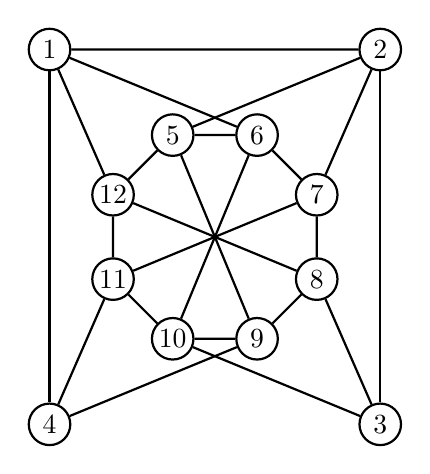
\begin{tikzpicture}[scale=1.4]
    \tikzstyle{edge}=[draw=black,thick,-]
    \tikzstyle{node}=[circle,thick,draw=black,fill=white,minimum size=15pt,inner sep=0pt]

    \def\x{0.382683}
    \def\y{0.923879}

    \def\X{1.5}
    \def\Y{1.7}

    \node[node] (x1)  at (-\X, \Y) {$1$};
    \node[node] (x2)  at ( \X, \Y) {$2$};
    \node[node] (x3)  at ( \X,-\Y) {$3$};
    \node[node] (x4)  at (-\X,-\Y) {$4$};
    \node[node] (x5)  at (-\x, \y) {$5$};
    \node[node] (x6)  at ( \x, \y) {$6$};
    \node[node] (x7)  at ( \y, \x) {$7$};
    \node[node] (x8)  at ( \y,-\x) {$8$};
    \node[node] (x9)  at ( \x,-\y) {$9$};
    \node[node] (x10) at (-\x,-\y) {$10$};
    \node[node] (x11) at (-\y,-\x) {$11$};
    \node[node] (x12) at (-\y, \x) {$12$};

    \path[edge] (x1) -- (x2);
    \path[edge] (x1) -- (x4);
    \path[edge] (x1) -- (x6);
    \path[edge] (x1) -- (x12);

    \path[edge] (x2) -- (x3);
    \path[edge] (x2) -- (x5);
    \path[edge] (x2) -- (x7);

    \path[edge] (x3) -- (x8);
    \path[edge] (x3) -- (x10);

    \path[edge] (x4) -- (x9);
    \path[edge] (x4) -- (x11);

    \path[edge] (x5) -- (x6);
    \path[edge] (x6) -- (x7);
    \path[edge] (x7) -- (x8);
    \path[edge] (x8) -- (x9);
    \path[edge] (x9) -- (x10);
    \path[edge] (x10) -- (x11);
    \path[edge] (x11) -- (x12);
    \path[edge] (x12) -- (x5);

    \path[edge] (x5) -- (x9);
    \path[edge] (x6) -- (x10);
    \path[edge] (x7) -- (x11);
    \path[edge] (x8) -- (x12);
\end{tikzpicture}


            \end{center}
        \end{column}
        \begin{column}[r]{0.4\textwidth}
            \pause
            \begin{center}
                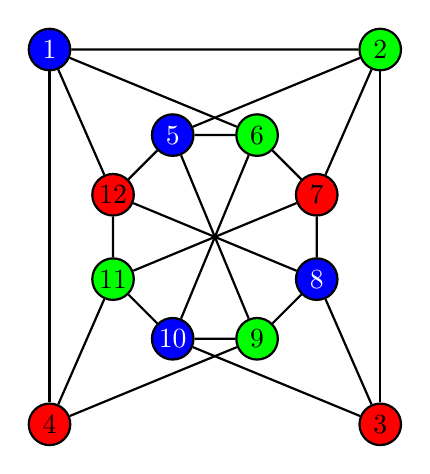
\begin{tikzpicture}[scale=1.4]
    \tikzstyle{edge}=[draw=black,thick,-]
    \tikzstyle{node}=[circle,thick,draw=black,fill=white,minimum size=15pt,inner sep=0pt]

    \tikzstyle{red}=[text=black,fill=red]
    \tikzstyle{green}=[text=black,fill=green]
    \tikzstyle{blue}=[text=white,fill=blue]

    \def\x{0.382683}
    \def\y{0.923879}

    \def\X{1.5}
    \def\Y{1.7}

    \node[node,blue]  (x1)  at (-\X, \Y) {$1$};
    \node[node,green] (x2)  at ( \X, \Y) {$2$};
    \node[node,red]   (x3)  at ( \X,-\Y) {$3$};
    \node[node,red]   (x4)  at (-\X,-\Y) {$4$};
    \node[node,blue]  (x5)  at (-\x, \y) {$5$};
    \node[node,green] (x6)  at ( \x, \y) {$6$};
    \node[node,red]   (x7)  at ( \y, \x) {$7$};
    \node[node,blue]  (x8)  at ( \y,-\x) {$8$};
    \node[node,green] (x9)  at ( \x,-\y) {$9$};
    \node[node,blue]  (x10) at (-\x,-\y) {$10$};
    \node[node,green] (x11) at (-\y,-\x) {$11$};
    \node[node,red]   (x12) at (-\y, \x) {$12$};

    \path[edge] (x1) -- (x2);
    \path[edge] (x1) -- (x4);
    \path[edge] (x1) -- (x6);
    \path[edge] (x1) -- (x12);

    \path[edge] (x2) -- (x3);
    \path[edge] (x2) -- (x5);
    \path[edge] (x2) -- (x7);

    \path[edge] (x3) -- (x8);
    \path[edge] (x3) -- (x10);

    \path[edge] (x4) -- (x9);
    \path[edge] (x4) -- (x11);

    \path[edge] (x5) -- (x6);
    \path[edge] (x6) -- (x7);
    \path[edge] (x7) -- (x8);
    \path[edge] (x8) -- (x9);
    \path[edge] (x9) -- (x10);
    \path[edge] (x10) -- (x11);
    \path[edge] (x11) -- (x12);
    \path[edge] (x12) -- (x5);

    \path[edge] (x5) -- (x9);
    \path[edge] (x6) -- (x10);
    \path[edge] (x7) -- (x11);
    \path[edge] (x8) -- (x12);
\end{tikzpicture}


            \end{center}
        \end{column}
    \end{columns}
\end{frame}

\begin{frame}
    \frametitle{The first example}
    \framesubtitle{Graph coloring with Gr\"{o}bner bases (1)}

    Given a graph $\mathcal{G}(V, E)$. We write two sets of equations:
    \begin{itemize}
        \item $I_k$ --- allow one of $k$ colors per vertex
            \begin{equation*}
                I_k = \{ x_i^k - 1 : i \in V \}
            \end{equation*}\pause
        \item $I_{\mathcal{G}}$ --- adjacent vertices have different colors assigned
            \begin{equation*}
                I_{\mathcal{G}} = \{ x_{i}^{k-1} + x_{i}^{k-2} x_{j} + \ldots + x_{i} x_{j}^{k-2} + x_{j}^{k-1} : (i, j) \in E \}
            \end{equation*}
    \end{itemize}
    \pause
    Next we solve $I_k \cup I_{\mathcal{G}}$ using the Gr\"{o}ebner bases method.
\end{frame}

\begin{frame}
    \frametitle{The first example}
    \framesubtitle{Graph coloring with Gr\"{o}bner bases (2)}

    \begin{columns}
        \begin{column}[l]{0.4\textwidth}
            \scriptsize
            \begin{align*}
                \{& \structure{x_{1}} + x_{11} + x_{12},              \\
                  & \structure{x_{2}} - x_{11},                       \\
                  & \structure{x_{3}} - x_{12},                       \\
                  & \structure{x_{4}} - x_{12},                       \\
                  & \structure{x_{5}} + x_{11} + x_{12},              \\
                  & \structure{x_{6}} - x_{11},                       \\
                  & \structure{x_{7}} - x_{12},                       \\
                  & \structure{x_{8}} + x_{11} + x_{12},              \\
                  & \structure{x_{9}} - x_{11},                       \\
                  & \structure{x_{10}} + x_{11} + x_{12},             \\
                  & \structure{x_{11}}^2 + x_{11} x_{12} + x_{12}^2,  \\
                  & \structure{x_{12}}^3 - 1 \}
            \end{align*}
        \end{column}
        \begin{column}[r]{0.4\textwidth}
            \begin{center}
                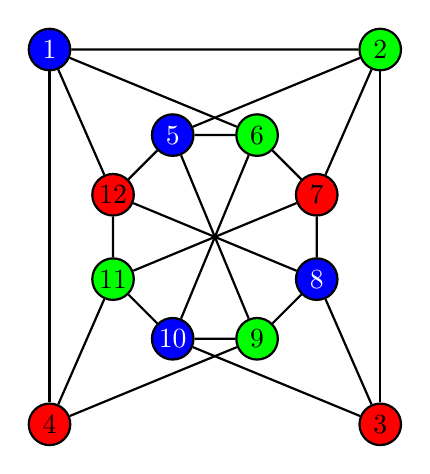
\begin{tikzpicture}[scale=1.4]
    \tikzstyle{edge}=[draw=black,thick,-]
    \tikzstyle{node}=[circle,thick,draw=black,fill=white,minimum size=15pt,inner sep=0pt]

    \tikzstyle{red}=[text=black,fill=red]
    \tikzstyle{green}=[text=black,fill=green]
    \tikzstyle{blue}=[text=white,fill=blue]

    \def\x{0.382683}
    \def\y{0.923879}

    \def\X{1.5}
    \def\Y{1.7}

    \node[node,blue]  (x1)  at (-\X, \Y) {$1$};
    \node[node,green] (x2)  at ( \X, \Y) {$2$};
    \node[node,red]   (x3)  at ( \X,-\Y) {$3$};
    \node[node,red]   (x4)  at (-\X,-\Y) {$4$};
    \node[node,blue]  (x5)  at (-\x, \y) {$5$};
    \node[node,green] (x6)  at ( \x, \y) {$6$};
    \node[node,red]   (x7)  at ( \y, \x) {$7$};
    \node[node,blue]  (x8)  at ( \y,-\x) {$8$};
    \node[node,green] (x9)  at ( \x,-\y) {$9$};
    \node[node,blue]  (x10) at (-\x,-\y) {$10$};
    \node[node,green] (x11) at (-\y,-\x) {$11$};
    \node[node,red]   (x12) at (-\y, \x) {$12$};

    \path[edge] (x1) -- (x2);
    \path[edge] (x1) -- (x4);
    \path[edge] (x1) -- (x6);
    \path[edge] (x1) -- (x12);

    \path[edge] (x2) -- (x3);
    \path[edge] (x2) -- (x5);
    \path[edge] (x2) -- (x7);

    \path[edge] (x3) -- (x8);
    \path[edge] (x3) -- (x10);

    \path[edge] (x4) -- (x9);
    \path[edge] (x4) -- (x11);

    \path[edge] (x5) -- (x6);
    \path[edge] (x6) -- (x7);
    \path[edge] (x7) -- (x8);
    \path[edge] (x8) -- (x9);
    \path[edge] (x9) -- (x10);
    \path[edge] (x10) -- (x11);
    \path[edge] (x11) -- (x12);
    \path[edge] (x12) -- (x5);

    \path[edge] (x5) -- (x9);
    \path[edge] (x6) -- (x10);
    \path[edge] (x7) -- (x11);
    \path[edge] (x8) -- (x12);
\end{tikzpicture}


            \end{center}
        \end{column}
    \end{columns}
\end{frame}

\begin{frame}[fragile]
    \frametitle{The first example}
    \framesubtitle{Graph coloring with Gr\"{o}bner bases in SymPy}

    \begin{python}
In [1]: V = range(1, 12+1)
In [2]: E = [(1,2),(2,3),(1,4),(1,6),(1,12),(2,5),(2,7),
(3,8),(3,10),(4,11),(4,9),(5,6),(6,7),(7,8),(8,9),(9,10),
(10,11),(11,12),(5,12),(5,9),(6,10),(7,11),(8,12)]

In [3]: X = [ Symbol('x' + str(i)) for i in V ]
In [4]: Z = [ (X[i-1], X[j-1]) for i, j in E ]

In [5]: U = [ x**3 - 1 for x in X ]
In [6]: V = [ x**2 + x*y + y**2 for x, y in Z ]

In [7]: G = groebner(U + V, X, order='lex')

In [8]: G != [1]
Out[8]: True
\end{python}


\end{frame}

\begin{frame}[fragile]
    \frametitle{A comparison with other systems}
    \framesubtitle{Graph coloring with Gr\"{o}bner bases in Maxima}

    \begin{maxima}
(i1) load(grobner);

(i2) E: [[1,2],[2,3],[1,4],[1,6],[1,12],[2,5],[2,7],[3,8],
[3,10],[4,11],[4,9],[5,6],[6,7],[7,8],[8,9],[9,10],[10,11],
[11,12],[5,12],[5,9],[6,10],[7,11],[8,12]];

(i3) X: makelist(concat("x", i), i, 1, 12);

(i4) U: makelist(X[i]^3 - 1, i, 1, 12);
(i5) V: [];

(i6) for e in E do
        V: endcons(X[e[1]]^2 + X[e[1]]*X[e[2]] + X[e[2]]^2, V);

(i7) G: poly_reduced_grobner(append(U, V), X);

(i8) is(notequal(G, [1]));
(o8) true
\end{maxima}


\end{frame}

\begin{frame}[fragile]
    \frametitle{A comparison with other systems}
    \framesubtitle{Graph coloring with Gr\"{o}bner bases in Axiom}

    \begin{python}
(1) -> E := [[1,2],[2,3],[1,4],[1,6],[1,12],[2,5],[2,7],
[3,8],[3,10],[4,11],[4,9],[5,6],[6,7],[7,8],[8,9],[9,10],
[10,11],[11,12],[5,12],[5,9],[6,10],[7,11],[8,12]];

(2) -> X := [ concat("x", i::String)::Symbol for i in 1..12 ];
(3) -> Z := [ [X.(e.1), X.(e.2)] for e in E ];

(4) -> U := [ x**3 - 1 for x in X ];
(5) -> V := [ z.1**2 + z.1*z.2 + z.2**2 for z in Z];

(6) -> G := groebner([ w::DMP(X, INT) for w in concat(U, V) ]);

(7) -> (G ~= [1]) @ Boolean
   (7) true
\end{python}


\end{frame}

\begin{frame}[fragile]
    \frametitle{A comparison with other systems}
    \framesubtitle{Graph coloring with Gr\"{o}bner bases in Mathematica}

    \begin{mathematica}
In[1]:= Unprotect[E];
In[2]:= E := {{1,2},{2,3},{1,4},{1,6},{1,12},{2,5},{2,7},
{3,8},{3,10},{4,11},{4,9},{5,6},{6,7},{7,8},{8,9},{9,10},
{10,11},{11,12},{5,12},{5,9},{6,10},{7,11},{8,12}}

In[3]:= X := Table[Symbol["x" <> ToString[i]], {i,1,n}]
In[4]:= h[{i_, j_}] := X[[i]]^2 + X[[i]] X[[j]] + X[[j]]^2

In[5]:= U := Map[(#^3-1)&, X]
In[6]:= V := Map[h, E]

In[7]:= G := GroebnerBasis[Join[U, V], X]

In[8]:= G != {1}
Out[8]= True
\end{mathematica}


\end{frame}

\begin{frame}[fragile]
    \frametitle{And what about the speed of computations?}
    \framesubtitle{In the case of our example \ldots}

    \begin{center}
        \begin{tabular}{l|llll} \toprule
                 & SymPy & Maxima & Axiom & Mathematica \\ \midrule
        Time [s] & 15.4  & 17.6   & 3.6   & 0.34        \\ \bottomrule
        \end{tabular}
    \end{center}
\end{frame}

\begin{frame}
    \begin{center}
        \vskip+0.5cm
        \textbf{\LARGE Thank you for your attention!}
        \linebreak
        \vskip+0.5cm
        
\includegraphics[scale=0.2]{images/sympy-logo.pdf}
    \end{center}
\end{frame}

\end{document}

